\documentclass[conference]{IEEEtran}
\IEEEoverridecommandlockouts
%\documentclass[a4paper,12pt]{article}

\usepackage{balance}
\usepackage{graphicx}
\usepackage{booktabs}
\usepackage{relsize}
\usepackage{pgfplots}
\usepackage{tabularx}
\usepackage{gensymb}
\usepackage{caption}
\usepackage{listings}
\usepackage{babel}
\usepackage{siunitx}
\usepackage{url}
\usepackage{subcaption}
\usepackage{comment}
\usepackage{tikz}


\usepackage[utf8]{inputenc}
\usepackage{amsmath}
\usepackage{hyperref}

%neue pacages vom neuen Template
\usepackage{cite}
\usepackage{amssymb,amsfonts} %hier vorher: \usepackage{amsmath,amssymb,amsfonts}
\usepackage{algorithmic}
\usepackage{textcomp}
\usepackage{xcolor}
\usepackage{epstopdf}
\usepackage{multirow}
\usepackage{blindtext}
\pgfplotsset{compat=1.18}
\title{\textbf{Shortpaper:} IoT-NDN: An IoT Architecture via Named Data
Netwoking (NDN)\\}
\author{Leonard Boetefuer}
\date{\today}


\begin{document}

\maketitle

\begin{abstract}
als Leztes
\end{abstract}

\section{Introduction}
als vorleztes
\section{Related Work}
XYZTEST2
\section{Analysis of IoT and NDN}
This section will talk about the limitations of IoT devices and the challenges of the current Internet architecture.
\subsection{The connectivity of IoT devices:}
Currently IoT devices use server-client or host-to-host connection to connect. 
In the server-client architecture every client has to communicate to the server and with a billion devices the server will be a massive bottleneck. In the host-host architecture, every host has to communicate to every other host. This results in exponential resource consumption.
The server-client and the host-to-host model both need IP addresses for every single device, which is not possible with a billion devices.
%check the ip adresses
%NDN solves the IP shortage and it is de-central helps with the bottleneck

\subsection{Technological Standards:}
The crucial standards are for the network protocols, the communication protocols, and the data aggregation. 
The challenge is that 
%überarbeiten 


\subsection{Mobility:}
The amount of mobile devices is rising and so are the challenges. The technologies of the mobile devices are divers and the IoT systems need to keep that in mind.

%Quelle 14 und 15

\subsection{Complexity and Integration Issues:}
IoT systems are composed of many different APIs (Application Programming Interfaces), protocols and platforms. 
%APIs expeccially are not desined with the resource limitations of IoT devices in mind. 
% maybe add that later
The integration of new technologies in the system is very complicated because of all the different combinations. The IoT system should consider the resource limitation of its components.




\section{Architecture of IoT-NDN System}
\section{Conclusion}

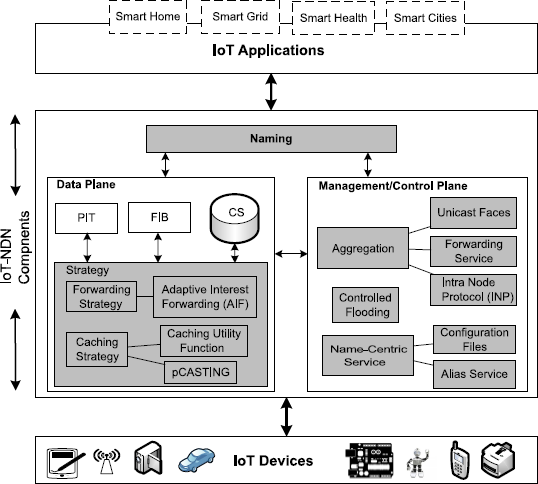
\includegraphics[width=0.5\textwidth]{IoT-NDN_System_architecture_and_its_components.png}\\
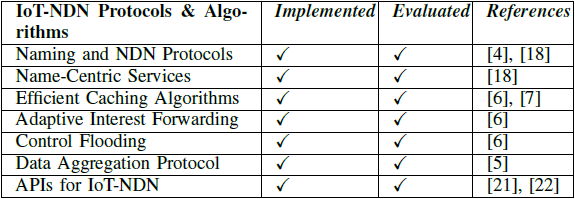
\includegraphics[width=0.5\textwidth]{IMPLEMENTED_AND_TESTED_PROTOCOLS_AND_ALGORITHMS_IN_IOT-NDN.png}\\
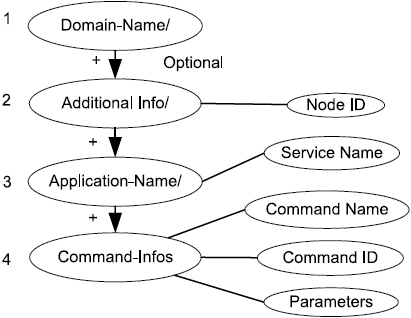
\includegraphics[width=0.5\textwidth]{Name_Structure_of_the_suggested_Approach.png}\\







%\subsection{Units}
% \begin{itemize}
% \item Related Work
% \item Analysis of IoT and NDN\\
%     A$)$ Challenges of IoT\\
%     \begin{enumerate}
%         \item The connection of IoT \\
%         the current paradigm are not usable for million or billions of devices.\\
%         The server-client architecture forces every device to communicate to the server first
%         and in the host-to-host architecture every device needs its own IP-adress.
        
%         \item Technology Standards\\
%         the current IoT technological standards have a problem with the aggregation of data.
%         the Data hase overhead to prevent data-aggregation, but the overhead consumes more energy and memory.
%         %nochmal angucken
        
%         \item Mobility\\
        
        
%         \item Complexity of Integration Issues
%     \end{enumerate}
%     B$)$ NDN for IoT\\
%     \begin{enumerate}
%         \item NDN Packet Lenght
%         \item Caching in IoT/NDN
%         \item Data Aggregation in Wireless Networks:
%         \item Naming Problems in Wirless Networks
%         \item Routing Scalability in NDN:
%     \end{enumerate}
% \item Architecture of IoT-NDN System\\
%     graphics and stuff\\
%     A$)$ Naming\\
%     B$)$ Management and Control Plane\\
%     \begin{itemize}
%         \item Aggregation
%         \item Controlled Flooding
%         \item Name-Centric Service
%     \end{itemize}
%     C$)$ Data PLane\\
%     \begin{itemize}
%         \item Strategy-In-Network Caching
%         \item Strategy-Forwarding
%     \end{itemize}
    
% \end{itemize}

% related Work

% short introduction\\

% A$)$ Challenges 1-5\\



\section{References}
XYZ
\end{document}